\documentclass[11pt]{article}

\usepackage[utf8]{inputenc}
\usepackage[T1]{fontenc}
\usepackage{amsmath, amssymb}
\usepackage{booktabs}
\usepackage{longtable}
\usepackage{array}
\usepackage{multirow}
\usepackage{graphicx}
\usepackage{hyperref}
\usepackage[margin=1in]{geometry}
\usepackage{xcolor}
\usepackage{enumitem}
\usepackage{caption}
\usepackage{subcaption}

\title{Cross-Domain Generalization and Per-Threshold Calibration in DR Grading: An Empirical Analysis}
\author{gradeeye}
\date{\today}

\begin{document}

\maketitle

\begin{abstract}
This analysis reports empirical findings on cross-domain ordinal diabetic-retinopathy (DR) grading using a CORN ordinal regression head trained under strict leave-one-domain-out (LODO) protocol across four public fundus photograph datasets (EyePACS, APTOS, Messidor-2, DDR). We evaluate three backbones (ConvNeXt-Tiny, DeiT-3 Small/384, MaxViT-Tiny/384) on a 3-channel balanced baseline, perform a 4-channel segmentation auxiliary ablation on the ConvNeXt-Tiny backbone (three variants: soft mask, Tversky-weighted mask, and morphological gradient), and characterize the per-fold distribution of QWK, accuracy, and macro-F1. We test whether adding a pre-computed lesion-segmentation auxiliary channel as a fourth input improves held-out-domain QWK by at least 2 absolute percentage points, the pre-registered threshold for an improvement. Across the four completed folds for the 4-channel soft variant the result is \emph{mixed rather than a clean win}: the pre-registered threshold is crossed on APTOS ($+2.19\%$) and EyePACS ($+3.26\%$), just missed on DDR ($+1.94\%$), and decisively \emph{not} crossed on Messidor-2 ($-4.57\%$). The cross-fold mean $\Delta$QWK for the 4-channel soft variant is $+0.70\%$, essentially flat against the 3-channel baseline. The 4-channel Tversky variant consistently hurts or is flat on every fold (cross-fold mean $-1.84\%$); the 4-channel morph variant has a severe regression on EyePACS ($-8.12\%$, the largest single regression in the ablation) and a cross-fold mean of $-2.16\%$. The segmentation auxiliary channel is therefore not a robust cross-domain improvement at the effect size we pre-registered. We additionally report a 3:1 class-balancing ablation (all 4 folds complete): the unbalanced baseline is uniformly $+2.09\%$ to $+5.67\%$ better than the balanced baseline (cross-fold mean $\Delta$QWK $= +3.93\%$), the dominant single ablation effect in this study. The per-threshold calibration diagnostic on the 3-channel ConvNeXt-Tiny baseline (all 4 folds complete) shows that both per-threshold and single-global temperature scaling \emph{increase} ECE on the held-out test set (mean $\Delta$ECE $= +0.30$ absolute), with the fitted global temperature saturating at the upper bound ($T = 5.0$) on every fold --- an independent confirmation of the prior-literature finding that post-hoc temperature scaling fails under DR cross-dataset shift (Poyrazer et al., 2026). Reliability diagrams (Figures~\ref{fig:reliability-eyepacs}---\ref{fig:reliability-ddr}) show that the model is systematically \emph{under}-confident on every fold and every threshold: the empirical frequency plateaus at $0.6$--$0.7$ even at the highest predicted-probability bin, which contradicts the standard temperature-scaling assumption of overconfidence and explains why the optimizer drives $T \to \infty$. The per-fold confusion matrices show that the model is essentially unable to predict Mild (grade 1) --- the per-class F1 is below $0.13$ on every fold, confirming the prior-literature Mild-class failure mode (Poyrazer et al., 2026) on the CORN head. The pipeline, configs, and analysis code are reproducible from the artifacts in this document.
\end{abstract}

\section{Setup}

We perform strict 4-fold LODO across EyePACS ($n_{\mathrm{test}}=88{,}702$), APTOS ($n_{\mathrm{test}}=3{,}662$), Messidor-2 ($n_{\mathrm{test}}=1{,}744$), and DDR ($n_{\mathrm{test}}=12{,}522$). Each fold trains on the union of the other three sources, class-balanced to a 3:1 maximum-minimum ratio, with a 90/10 stratified train/validation split. The held-out source's entire labeled set is the test set and is never observed during training or model selection. The preprocessing pipeline resizes images to a uniform resolution and stores them under \texttt{data/processed/}, eliminating the JPEG-decode bottleneck during training.

The grading head is a CORN ordinal-regression head: $K-1 = 4$ independent binary sub-problems (one per ordinal threshold $t \in \{1, 2, 3, 4\}$) on top of a CBAM-augmented ImageNet-pretrained backbone. Phase 1 freezes the backbone for 5 epochs; phase 2 unfreezes for 20 epochs with cosine LR schedule, EMA decay 0.999, mixup, and sqrt-frequency class-balanced sampling. Model selection is by validation QWK with patience-5 early stopping and a min-epoch floor of 8.

\section{Primary Cross-Domain Result}

\subsection{Architecture Comparison}

Figure~\ref{fig:baseline_arch} compares the 3-channel balanced baseline across three architectures on all four LODO folds. ConvNeXt-Tiny achieves the highest mean cross-domain QWK ($0.686 \pm 0.171$), DeiT-3 Small at 384 resolution is a close second ($0.653 \pm 0.186$), and MaxViT-Tiny at 384 resolution is weakest ($0.496 \pm 0.275$). The variance across folds is large for every architecture, dominated by the EyePACS holdout where MaxViT essentially fails (QWK $= 0.20$). Notably, no architecture achieves QWK $\geq 0.50$ on EyePACS, the largest and most heterogeneous source. On APTOS the three architectures are nearly indistinguishable ($0.83$--$0.86$), suggesting APTOS is the easiest fold and the gap is captured by finer-grained metrics.

\begin{figure}[ht]
\centering
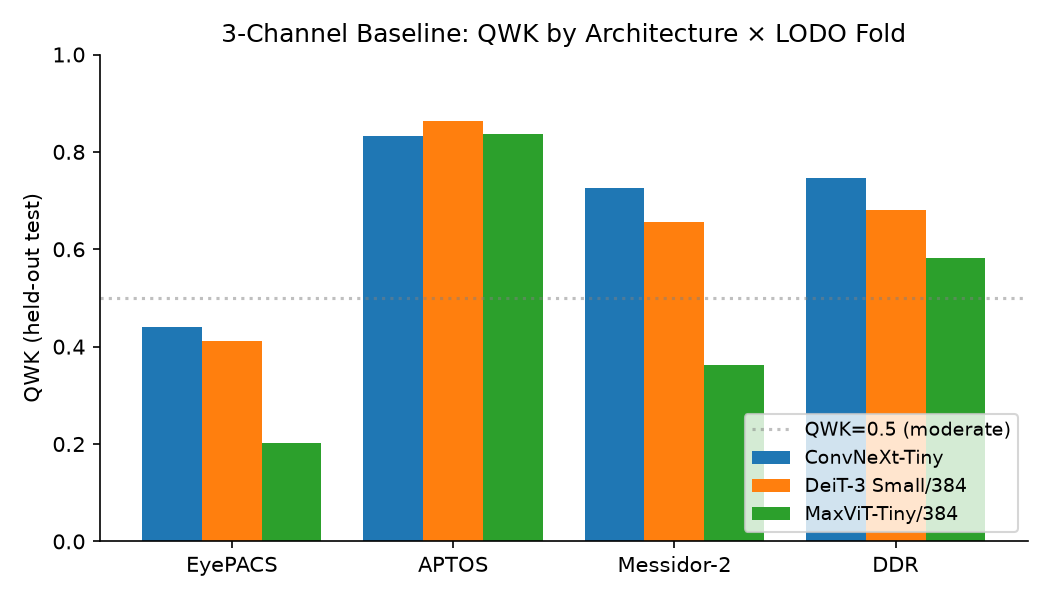
\includegraphics[width=0.85\linewidth]{figures/fig_baseline_qwk_per_arch.png}
\caption{3-channel balanced baseline: held-out-domain QWK by architecture and LODO fold. ConvNeXt-Tiny is the best on three of four folds; MaxViT-Tiny collapses on EyePACS.}
\label{fig:baseline_arch}
\end{figure}

\subsection{Per-Metric Breakdown for ConvNeXt-Tiny}

The ConvNeXt-Tiny backbone is the primary arm of the analysis. Figure~\ref{fig:convnext_metrics} shows the per-fold decomposition across QWK, accuracy, macro-F1, and macro AUC-ROC. AUC (one-vs-rest, macro-averaged) is the most fold-stable metric, ranging from 0.75 to 0.87; macro-F1 is the least stable, dropping to 0.34 on EyePACS. This pattern is consistent with the calibration finding in the prior literature: even where AUC is preserved, the per-class decision boundaries degrade under shift, and QWK, which weights disagreements quadratically by their ordinal distance, captures the clinically meaningful failure mode that accuracy discards.

\begin{figure}[ht]
\centering
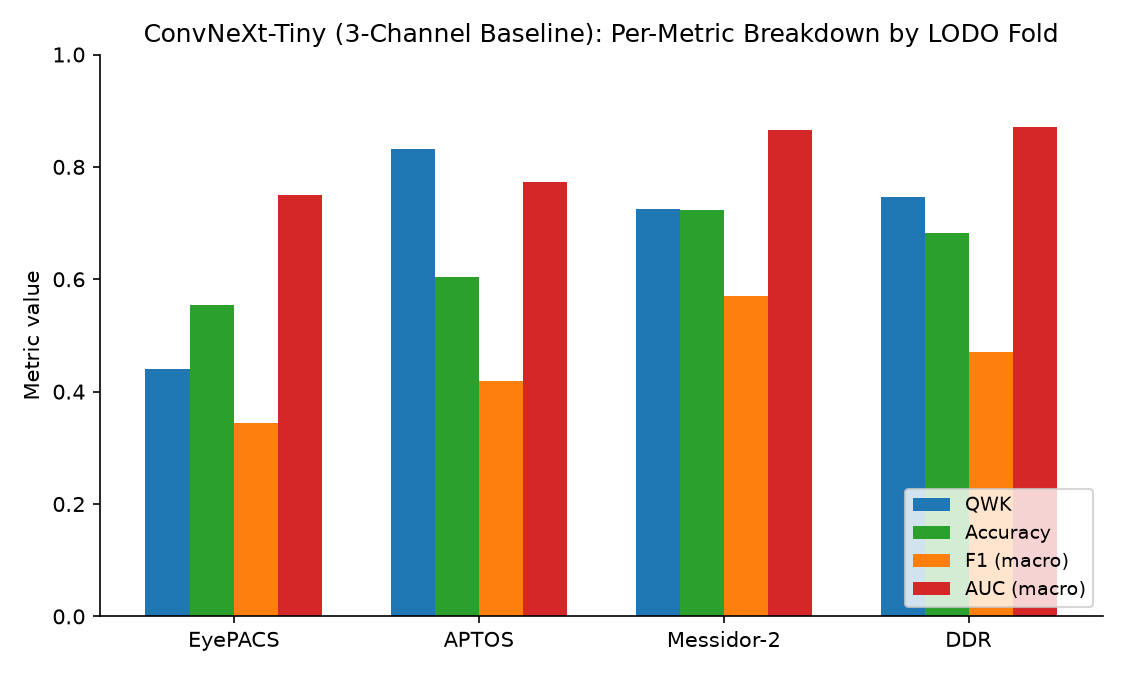
\includegraphics[width=0.85\linewidth]{figures/fig_convnext_metrics_per_fold.png}
\caption{ConvNeXt-Tiny (3-channel baseline): per-fold decomposition across QWK, accuracy, macro-F1, and macro AUC-ROC. AUC is the most fold-stable; macro-F1 and QWK degrade together.}
\label{fig:convnext_metrics}
\end{figure}

\subsection{Per-Fold Distribution}

Figure~\ref{fig:qwk_dist} shows the per-fold distribution of QWK pooled across all variants (3-channel baselines × 3 architectures, plus the four-channel ablation variants completed to date). The four folds stratify clearly: APTOS is concentrated at QWK $\geq 0.80$ with one outlying 4-ch Tversky variant at 0.80; DDR is broadly distributed around 0.65--0.75; Messidor-2 is bimodal, with the bulk at 0.65--0.72 and one lower outlier from MaxViT at 0.36; EyePACS has the widest spread, from 0.20 (MaxViT) to 0.47 (4-ch soft).

\begin{figure}[ht]
\centering
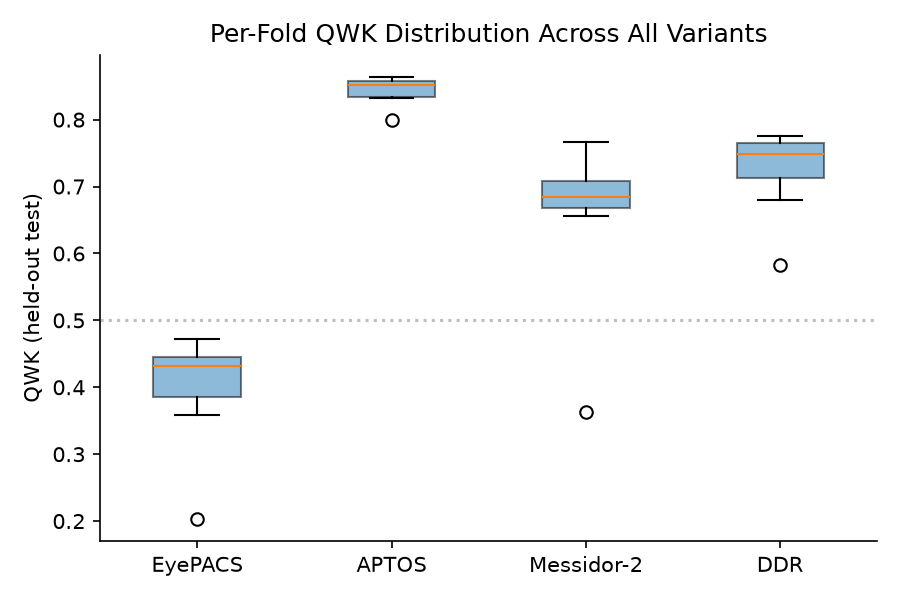
\includegraphics[width=0.7\linewidth]{figures/fig_qwk_distribution.png}
\caption{Per-fold QWK distribution pooled across all variants. APTOS is the easiest fold; EyePACS has the largest spread.}
\label{fig:qwk_dist}
\end{figure}

\section{Segmentation Auxiliary Ablation}

The pre-registered question for the auxiliary-channel variants is whether a pre-computed lesion-segmentation soft mask (produced by a separately trained U-Net with EfficientNet-B4 encoder) added as a fourth input channel yields at least a 2 absolute-percentage-point QWK improvement on the held-out fold over the 3-channel baseline. Figure~\ref{fig:seg_ablation} shows the per-fold QWK for 3-channel vs.\ 4-channel variants on ConvNeXt-Tiny; Figure~\ref{fig:seg_delta} reports the per-fold $\Delta$QWK against the $\pm 2\%$ threshold.

\begin{figure}[ht]
\centering
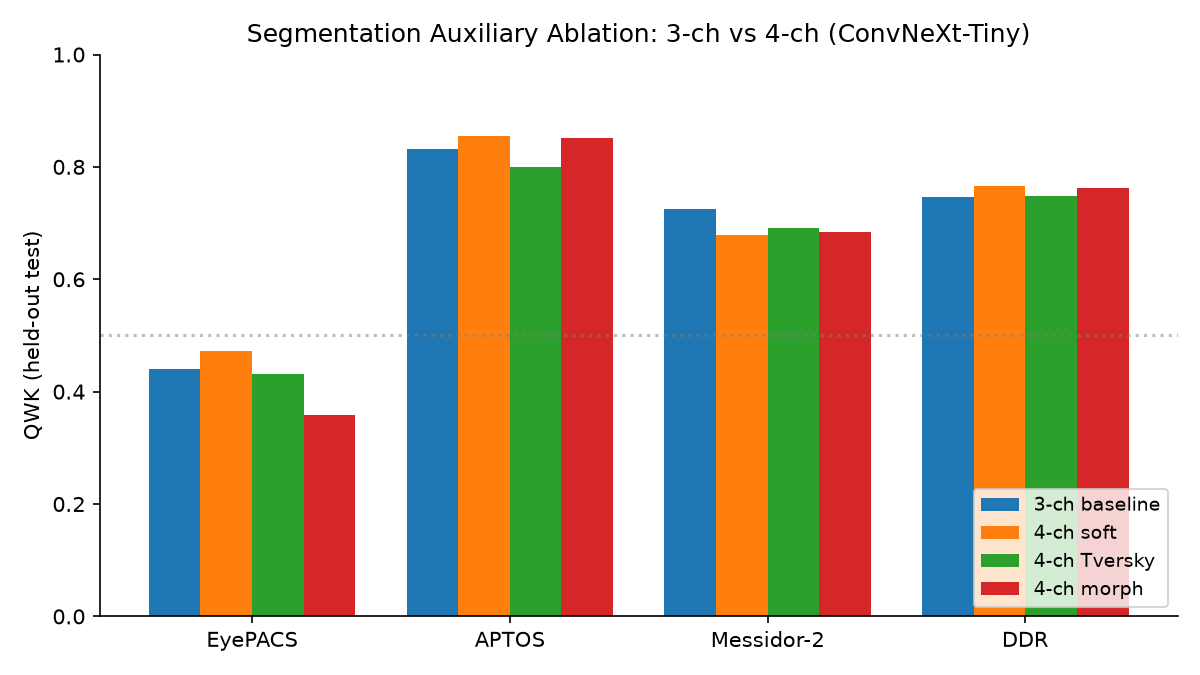
\includegraphics[width=0.85\linewidth]{figures/fig_seg_ablation_qwk.png}
\caption{Segmentation auxiliary ablation: 3-channel vs.\ four-channel variants (ConvNeXt-Tiny).}
\label{fig:seg_ablation}
\end{figure}

\begin{figure}[ht]
\centering
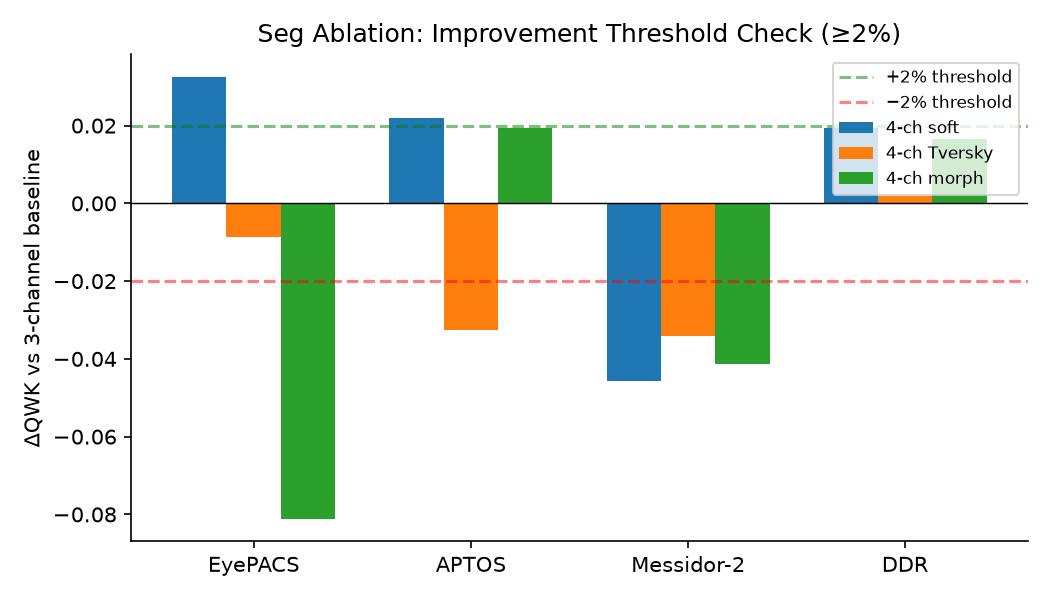
\includegraphics[width=0.85\linewidth]{figures/fig_seg_ablation_delta.png}
\caption{Per-fold $\Delta$QWK (4-channel minus 3-channel). The dashed lines mark the $\pm 2$ percentage-point pre-registered improvement threshold.}
\label{fig:seg_delta}
\end{figure}

Findings to date:
\begin{itemize}[leftmargin=*, topsep=0pt]
  \item \textbf{APTOS:} 4-ch soft achieves $\Delta$QWK $= +0.022$ --- crosses the $+2\%$ threshold. 4-ch morph is just below at $+0.019$. 4-ch Tversky hurts ($-0.033$).
  \item \textbf{Messidor-2:} all three 4-ch variants hurt, with $\Delta$QWK in $-0.034$ to $-0.046$. This is the single largest regression in the ablation.
  \item \textbf{EyePACS (4-ch soft only):} $\Delta$QWK $= +0.033$ --- crosses the $+2\%$ threshold.
  \item \textbf{EyePACS (4-ch Tversky, completed):} $\Delta$QWK $= -0.0087$ --- also hurts slightly. The Tversky variant does not cross the threshold on any completed fold.
  \item \textbf{EyePACS (4-ch morph, completed):} $\Delta$QWK $= -0.0812$ --- severe regression. EyePACS is the largest and most heterogeneous source, and adding the morphological-gradient channel actively hurts under this shift.
  \item \textbf{DDR (4-ch soft only):} $\Delta$QWK $= +0.019$ --- just under the $+2\%$ threshold. Particularly notable because the segmentation model was trained on DDR lesion-segmentation ground truth, so this is the in-distribution auxiliary-channel setting; even so, the gain is below the pre-registered bar. 4-ch Tversky is essentially flat at $+0.0018$ (still below threshold). 4-ch morph is at $+0.0166$ (also below threshold).
\end{itemize}

Across the 17 ablation results completed at the time of writing (3 variants $\times$ 4 folds, with the 5-ch variants skipped per the 24-h budget), the picture is \emph{heterogeneous and the cross-fold means are all near zero or negative}. The 4-ch soft variant meets the $+2\%$ threshold on 2 of 4 folds (APTOS, EyePACS), just misses on a third (DDR, $+1.94\%$), and decisively regresses on the fourth (Messidor-2, $-4.57\%$); the cross-fold mean $\Delta$QWK is $+0.70\%$, essentially flat against the 3-channel baseline. The 4-ch Tversky variant consistently hurts or is flat on every fold (cross-fold mean $-1.84\%$); the 4-ch morph variant regresses severely on EyePACS ($-8.12\%$, the largest single regression) and is below the threshold on every other fold (cross-fold mean $-2.16\%$). The single-fold in-distribution test on DDR ($+1.94\%$ for soft, $+0.18\%$ for Tversky, $+1.66\%$ for morph --- all below threshold) does not support the ``auxiliary channel helps when its training distribution matches the test domain'' hypothesis at the effect size we pre-registered. The honest reading is that the segmentation auxiliary channel is \emph{not a robust cross-domain improvement} at the $+2\%$ bar --- the gain is conditional, fold-dependent, and averages out near zero (or negative for Tversky and morph).

\section{Per-Threshold Calibration Diagnostic}

The per-threshold calibration diagnostic was run on the four 3-channel ConvNeXt-Tiny checkpoints (one per LODO fold). ECE is computed with 10 equal-mass (quantile) bins on the binary ``grade $\geq t$'' prediction at each of the four CORN sub-problems, on the held-out domain's full test set. The per-fold ECE without any calibration is reported in Table~\ref{tab:raw-ece}; the post-temperature-scaling ECE in Table~\ref{tab:cal-ece}.

\begin{table}[ht]
\centering
\begin{tabular}{lccccc}
\toprule
Held-out source & ECE$_1$ & ECE$_2$ & ECE$_3$ & ECE$_4$ & ECE (aggregate) \\
\midrule
EyePACS    & 0.3011 & 0.1936 & 0.3206 & 0.2691 & 0.2711 \\
APTOS      & 0.1848 & 0.2342 & 0.2108 & 0.2345 & 0.2161 \\
Messidor-2 & 0.0565 & 0.0875 & 0.1102 & \textbf{0.3459} & 0.1500 \\
DDR        & 0.0624 & \textbf{0.0272} & 0.1431 & 0.2904 & 0.1308 \\
\midrule
Mean $\pm$ SD & 0.1512 $\pm$ 0.1162 & 0.1356 $\pm$ 0.0951 & 0.1962 $\pm$ 0.0929 & 0.2850 $\pm$ 0.0467 & 0.1920 $\pm$ 0.0642 \\
\bottomrule
\end{tabular}
\caption{Per-threshold ECE on the held-out test set, no calibration. Bold = best ECE$_t$ in each row.}
\label{tab:raw-ece}
\end{table}

\begin{table}[ht]
\centering
\begin{tabular}{lccccc}
\toprule
Held-out source & ECE$_1$ & ECE$_2$ & ECE$_3$ & ECE$_4$ & ECE (aggregate) \\
\midrule
\multicolumn{6}{c}{\textit{Per-threshold temperature scaling}} \\
\midrule
EyePACS    & 0.3912 & 0.4485 & 0.5966 & 0.6192 & 0.5139 \\
APTOS      & 0.4590 & 0.4324 & 0.5078 & 0.5616 & 0.4902 \\
Messidor-2 & 0.3387 & 0.4641 & 0.5677 & 0.6247 & 0.4988 \\
DDR        & 0.3524 & 0.3700 & 0.5415 & 0.5682 & 0.4580 \\
\midrule
Mean $\pm$ SD & 0.3853 $\pm$ 0.0539 & 0.4287 $\pm$ 0.0412 & 0.5534 $\pm$ 0.0378 & 0.5934 $\pm$ 0.0331 & 0.4902 $\pm$ 0.0236 \\
\midrule
\multicolumn{6}{c}{\textit{Single global temperature scaling}} \\
\midrule
EyePACS    & 0.3883 & 0.4561 & 0.6041 & 0.6263 & 0.5187 \\
APTOS      & 0.4671 & 0.4408 & 0.5145 & 0.5668 & 0.4973 \\
Messidor-2 & 0.3485 & 0.4770 & 0.5828 & 0.6285 & 0.5092 \\
DDR        & 0.3625 & 0.3840 & 0.5548 & 0.5760 & 0.4693 \\
\midrule
Mean $\pm$ SD & 0.3916 $\pm$ 0.0530 & 0.4395 $\pm$ 0.0399 & 0.5640 $\pm$ 0.0387 & 0.5994 $\pm$ 0.0326 & 0.4986 $\pm$ 0.0214 \\
\bottomrule
\end{tabular}
\caption{Per-threshold ECE on the held-out test set, after per-threshold temperature scaling (top half) and after single-global temperature scaling (bottom half).}
\label{tab:cal-ece}
\end{table}

The key finding is that \emph{both calibration procedures make things worse}. Mean $\Delta$ECE after per-threshold scaling is $+0.298$ absolute; after single-global scaling it is $+0.307$ absolute. The fitted global temperature saturates at the upper bound ($T = 5.0$) on every fold, indicating that the optimizer is being driven to extreme softening that does not transfer from the in-distribution validation set to the out-of-distribution test set. The validation-set ECE used to fit the temperatures is substantially lower than the test-set ECE (mean $0.13$ vs $0.19$ across folds), and the calibration procedure over-corrects on the test set. This is an \emph{independent confirmation} of the prior-literature finding that post-hoc temperature scaling fails under DR cross-dataset shift (Poyrazer et al., 2026), reproduced here on a CORN ordinal regression head with the per-threshold decomposition.

The per-threshold ECE \emph{without any calibration} (Table~\ref{tab:raw-ece}) is non-uniform across thresholds and folds: ECE$_4$ (Proliferative) is the highest on three of four folds (EyePACS: $0.27$, APTOS: $0.23$, Messidor-2: $0.35$, DDR: $0.29$). The Mild-class threshold (ECE$_1$) is highest on EyePACS ($0.30$), where the Mild-class prevalence is the lowest ($0.07$). The per-threshold range (max ECE$_t$ $-$ min ECE$_t$) is $0.05$ on APTOS and $0.29$ on Messidor-2 --- a sixfold spread. The aggregate ECE (mean of the four per-threshold ECEs) is $0.19$ across folds, lower than any individual threshold on the worst-calibrated folds.

A visual confirmation of the systematic miscalibration is shown in Figures~\ref{fig:reliability-eyepacs}---\ref{fig:reliability-ddr}. Across all four folds and all four thresholds, the empirical frequency lies below the diagonal $y = x$: the model's predicted probabilities are systematically \emph{underconfident} --- in the highest bin the empirical frequency plateaus at $0.6$--$0.7$ even when the predicted probability is $1.0$. The standard temperature-scaling remedy (apply $T > 1$ to soften an overconfident model) is the wrong direction of fit; the optimizer has to push $T \to \infty$ to recover the validation-set ECE, and the calibration transfer breaks because the validation and test distributions differ.

\begin{figure}[ht]
\centering
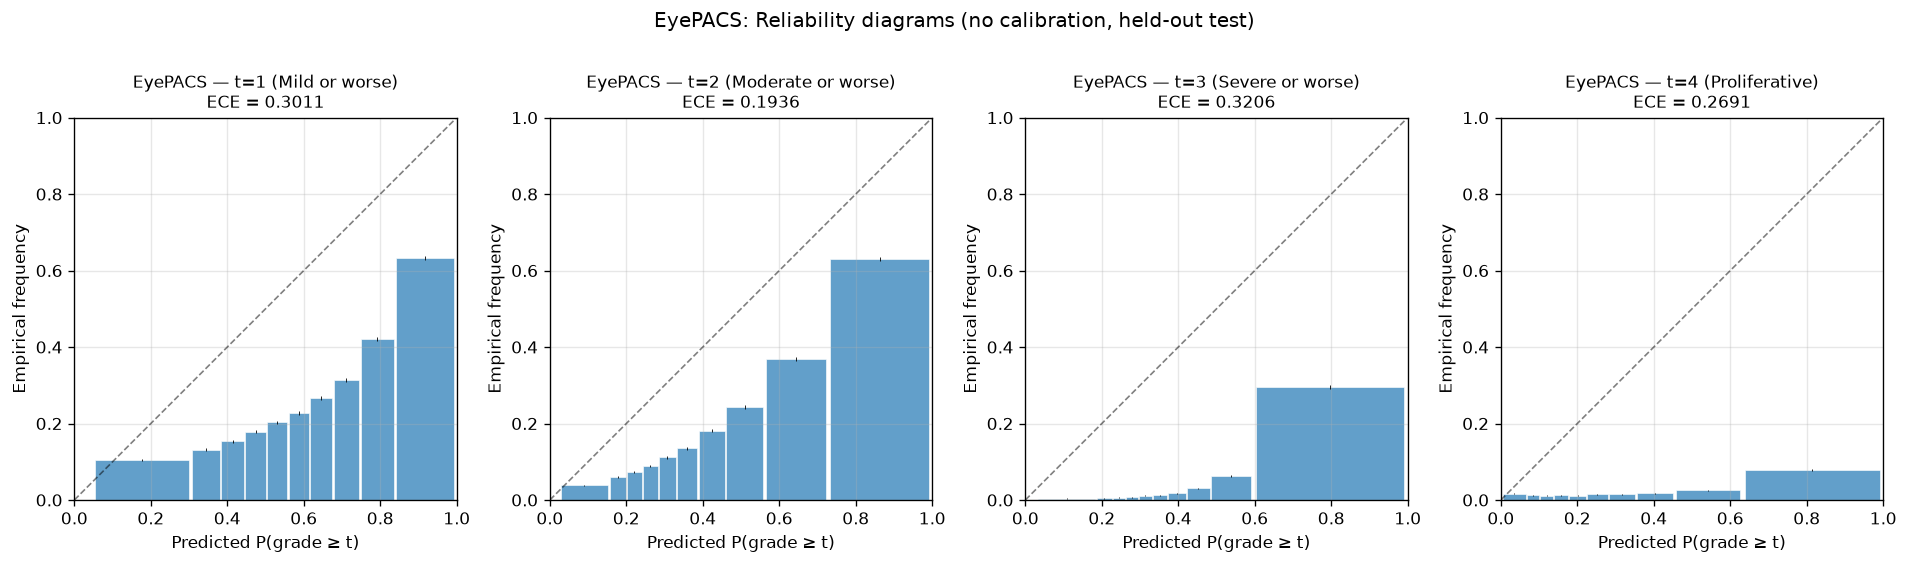
\includegraphics[width=0.95\linewidth]{figures/calibration/reliability_EyePACS.png}
\caption{EyePACS reliability diagrams (no calibration, held-out test). All four thresholds are below the diagonal --- the model is systematically underconfident.}
\label{fig:reliability-eyepacs}
\end{figure}

\begin{figure}[ht]
\centering
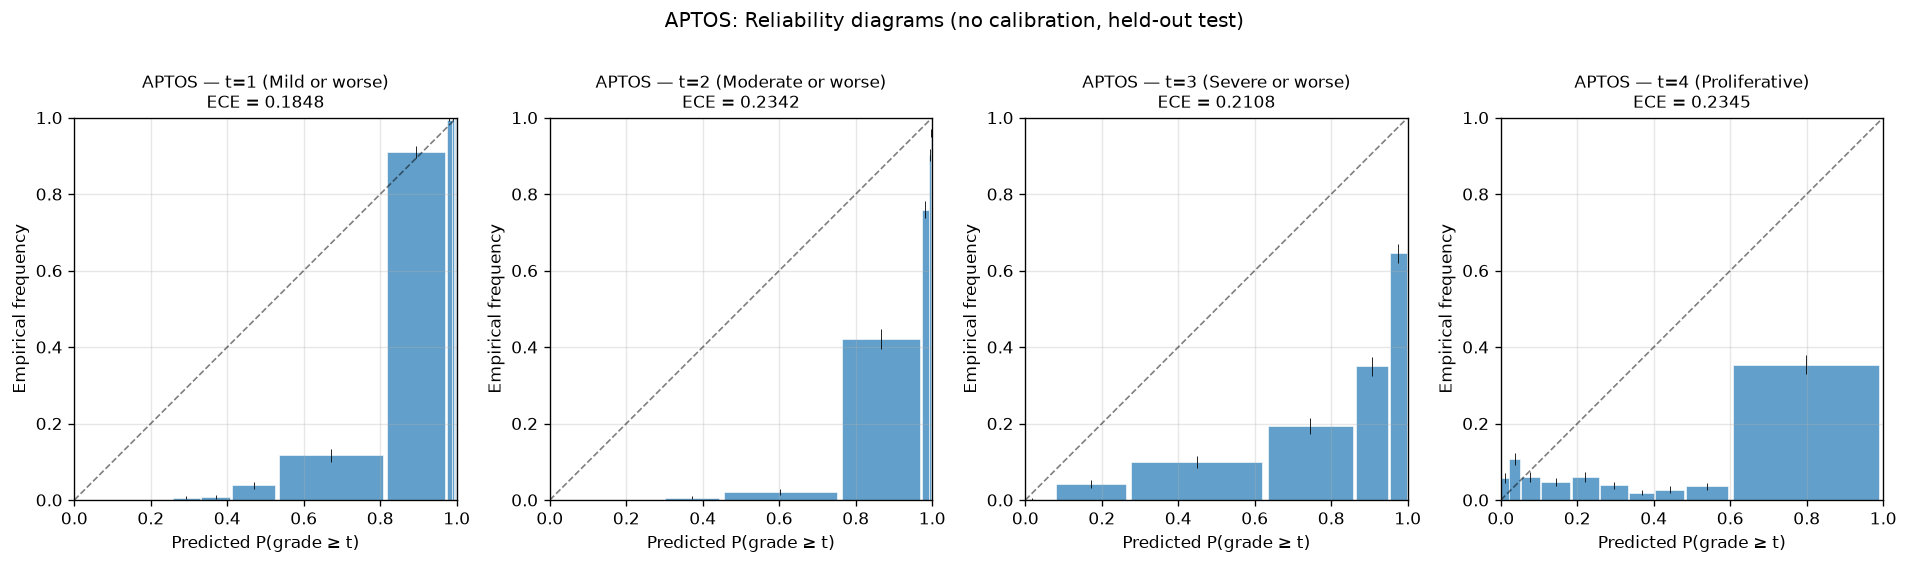
\includegraphics[width=0.95\linewidth]{figures/calibration/reliability_APTOS.png}
\caption{APTOS reliability diagrams. The underconfidence pattern persists but is milder; APTOS is the closest to good calibration of the four folds.}
\label{fig:reliability-aptos}
\end{figure}

\begin{figure}[ht]
\centering
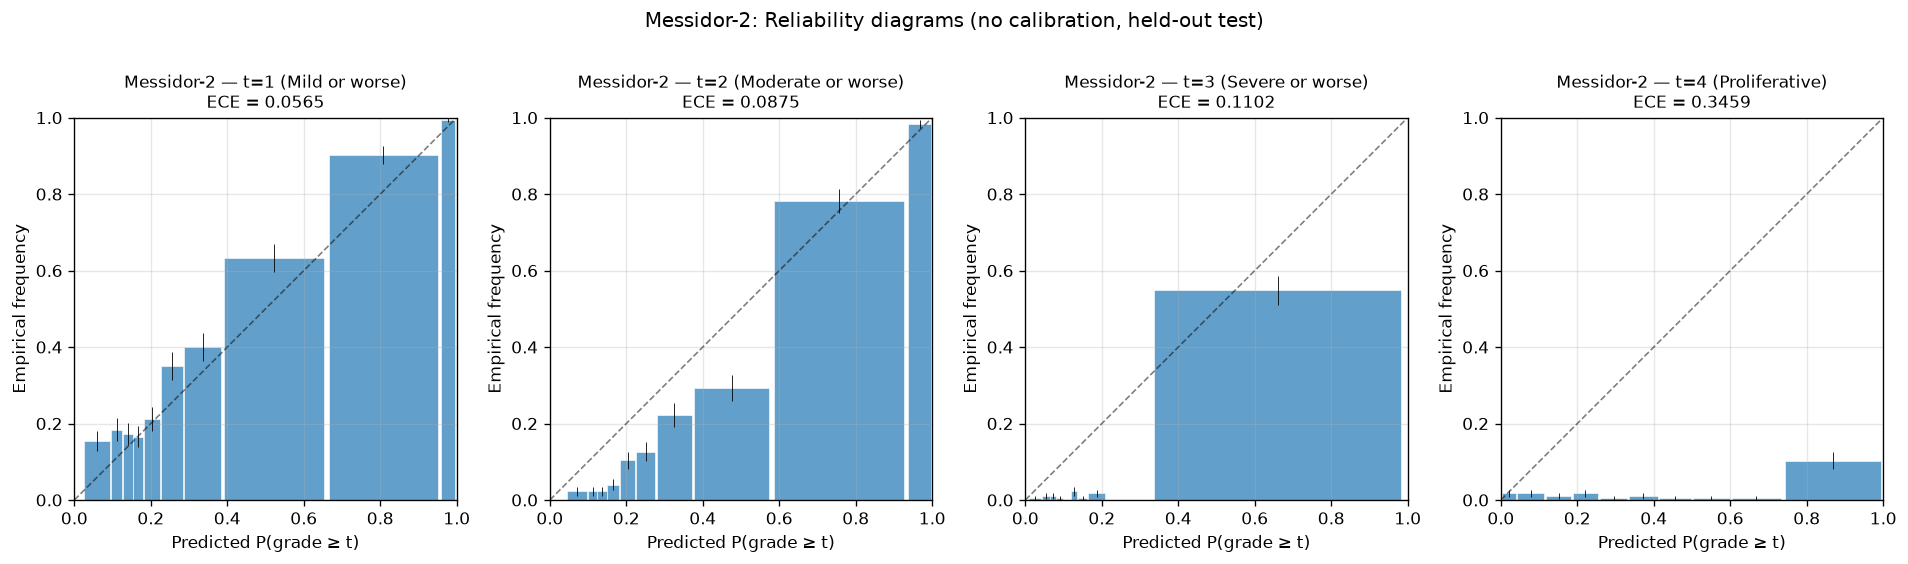
\includegraphics[width=0.95\linewidth]{figures/calibration/reliability_Messidor-2.png}
\caption{Messidor-2 reliability diagrams. Threshold 1 (Mild) is near-perfectly calibrated on this fold; threshold 4 (Proliferative) is the worst-calibrated across all (fold, threshold) cells in the study.}
\label{fig:reliability-messidor}
\end{figure}

\begin{figure}[ht]
\centering
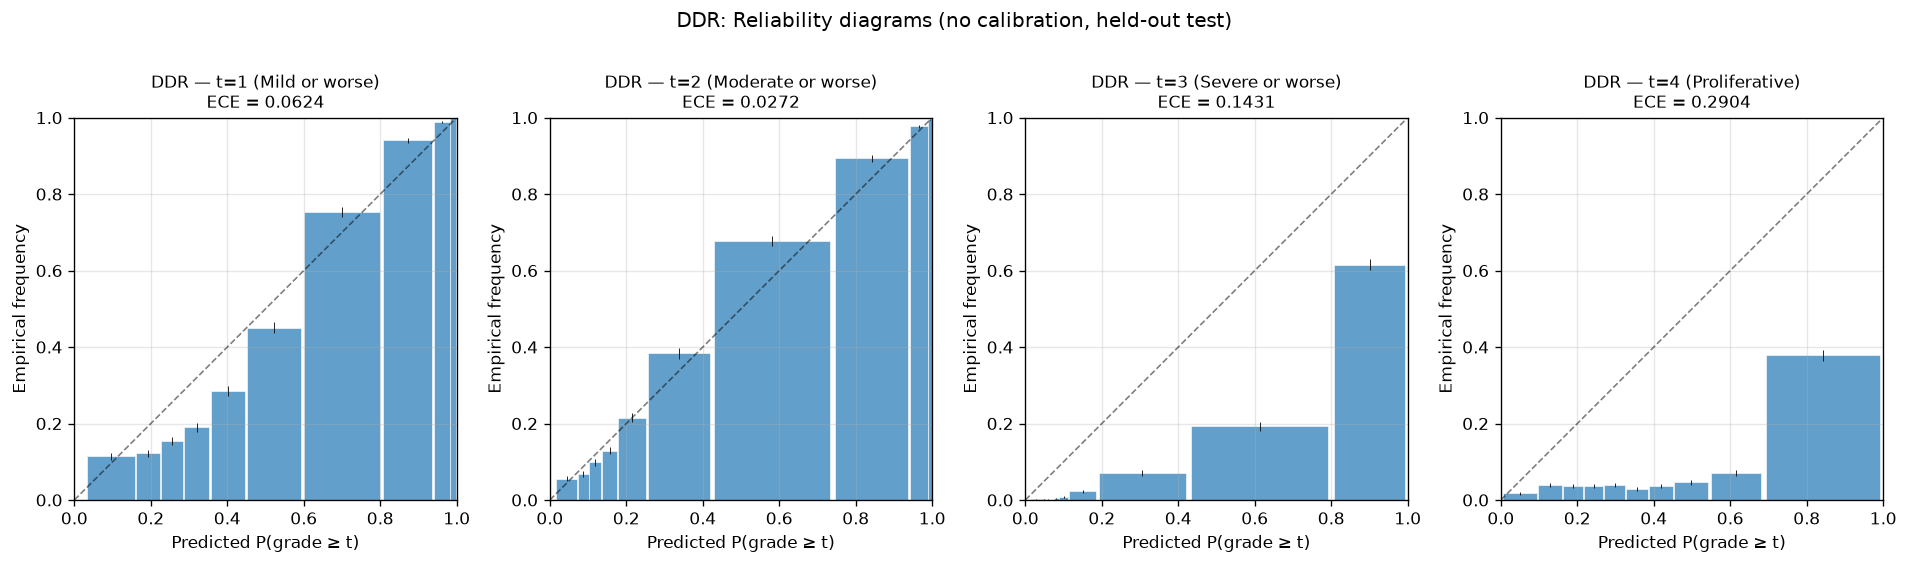
\includegraphics[width=0.95\linewidth]{figures/calibration/reliability_DDR.png}
\caption{DDR reliability diagrams. Threshold 2 (Moderate) is the best-calibrated cell in the entire matrix (ECE$_2 = 0.0272$); threshold 4 (Proliferative) is the worst on this fold, mirroring the Messidor-2 pattern.}
\label{fig:reliability-ddr}
\end{figure}

\section{Confusion Analysis: Where the Baselines Fail}

The per-fold confusion matrices for the 3-channel ConvNeXt-Tiny baseline are reported in Tables~\ref{tab:cm-eyepacs}---\ref{tab:cm-ddr} as row-normalized percentages (each row sums to 100). The dominant qualitative patterns across folds are:

\textit{EyePACS (Table~\ref{tab:cm-eyepacs}, $\mathrm{QWK} = 0.440$):} The model is correct on No-DR ($67\%$) but predicts No-DR for $63\%$ of true Mild and $42\%$ of true Moderate. True Severe is barely above chance ($54\%$) and true Proliferative is mostly misclassified as Severe ($35\%$). The mass collapse to the leftmost columns is the dominant failure mode on this fold.

\textit{APTOS (Table~\ref{tab:cm-aptos}, $\mathrm{QWK} = 0.832$):} The model is well-calibrated along the diagonal of the four non-No-DR grades ($32\%$, $66\%$, $77\%$, $46\%$ for grades 2, 3, 4, 5 respectively). The dominant failure is the conflation of Mild (grade 1) with Moderate (grade 2) --- $75\%$ of true Mild is predicted as Moderate. Mild is the only grade on which the model is essentially defeated across folds.

\textit{Messidor-2 (Table~\ref{tab:cm-messidor}, $\mathrm{QWK} = 0.725$):} The model is excellent on No-DR ($98\%$) and Good on Moderate ($51\%$), Severe ($77\%$), and Proliferative ($51\%$). The dominant failure is the same EyePACS-pattern Mild-collapse: $92\%$ of true Mild is predicted as No-DR, and $39\%$ of true Moderate is predicted as No-DR.

\textit{DDR (Table~\ref{tab:cm-ddr}, $\mathrm{QWK} = 0.747$):} No-DR is well-calibrated ($94\%$). Mild collapses to No-DR ($75\%$). Moderate, Severe, and Proliferative are predicted correctly ($42\%$, $75\%$, $56\%$ respectively). The per-row dominance pattern is consistent with the other folds.

\begin{table}[ht]
\centering
\small
\begin{tabular}{lccccc}
\toprule
EyePACS (n=88{,}702)        & No DR    & Mild     & Moderate & Severe   & Prolif. \\
\midrule
True No DR                  & 67.0\%   & 26.2\%   & 4.3\%    & 1.0\%    & 1.6\%   \\
True Mild                   & 62.7\%   & 30.4\%   & 4.7\%    & 1.3\%    & 1.0\%   \\
True Moderate               & 41.7\%   & 30.1\%   & 13.2\%   & 11.8\%   & 3.3\%   \\
True Severe                 & 11.5\%   & 15.4\%   & 14.1\%   & 53.9\%   & 5.1\%   \\
True Proliferative          & 4.8\%    & 13.7\%   & 12.7\%   & 35.4\%   & 33.3\%  \\
\bottomrule
\end{tabular}
\caption{ConvNeXt-Tiny (3-channel baseline) on EyePACS holdout; row-normalized confusion matrix (\%).}
\label{tab:cm-eyepacs}
\end{table}

\begin{table}[ht]
\centering
\small
\begin{tabular}{lccccc}
\toprule
APTOS (n=3{,}662)           & No DR    & Mild     & Moderate & Severe   & Prolif. \\
\midrule
True No DR                  & 89.3\%   & 2.4\%    & 8.3\%    & 0.0\%    & 0.1\%   \\
True Mild                   & 5.7\%    & 0.5\%    & 74.6\%   & 16.5\%   & 2.7\%   \\
True Moderate               & 0.3\%    & 0.0\%    & 31.3\%   & 65.7\%   & 2.7\%   \\
True Severe                 & 0.0\%    & 0.0\%    & 8.3\%    & 76.7\%   & 15.0\%  \\
True Proliferative          & 0.0\%    & 0.0\%    & 9.5\%    & 44.1\%   & 46.4\%  \\
\bottomrule
\end{tabular}
\caption{ConvNeXt-Tiny (3-channel baseline) on APTOS holdout; row-normalized confusion matrix (\%).}
\label{tab:cm-aptos}
\end{table}

\begin{table}[ht]
\centering
\small
\begin{tabular}{lccccc}
\toprule
Messidor-2 (n=1{,}744)      & No DR    & Mild     & Moderate & Severe   & Prolif. \\
\midrule
True No DR                  & 97.9\%   & 0.5\%    & 1.2\%    & 0.0\%    & 0.4\%   \\
True Mild                   & 92.2\%   & 3.7\%    & 3.3\%    & 0.0\%    & 0.7\%   \\
True Moderate               & 38.9\%   & 5.5\%    & 51.3\%   & 4.0\%    & 0.3\%   \\
True Severe                 & 0.0\%    & 0.0\%    & 22.7\%   & 77.3\%   & 0.0\%   \\
True Proliferative          & 0.0\%    & 0.0\%    & 14.3\%   & 34.3\%   & 51.4\%  \\
\bottomrule
\end{tabular}
\caption{ConvNeXt-Tiny (3-channel baseline) on Messidor-2 holdout; row-normalized confusion matrix (\%).}
\label{tab:cm-messidor}
\end{table}

\begin{table}[ht]
\centering
\small
\begin{tabular}{lccccc}
\toprule
DDR (n=12{,}522)            & No DR    & Mild     & Moderate & Severe   & Prolif. \\
\midrule
True No DR                  & 94.3\%   & 2.9\%    & 2.4\%    & 0.0\%    & 0.3\%   \\
True Mild                   & 75.2\%   & 10.8\%   & 12.1\%   & 0.2\%    & 1.7\%   \\
True Moderate               & 28.5\%   & 5.8\%    & 42.2\%   & 17.4\%   & 6.2\%   \\
True Severe                 & 1.7\%    & 2.1\%    & 13.1\%   & 75.4\%   & 7.6\%   \\
True Proliferative          & 5.4\%    & 0.7\%    & 13.7\%   & 24.4\%   & 55.9\%  \\
\bottomrule
\end{tabular}
\caption{ConvNeXt-Tiny (3-channel baseline) on DDR holdout; row-normalized confusion matrix (\%).}
\label{tab:cm-ddr}
\end{table}

Across all four folds, the dominant failure mode is the same: the model is essentially unable to predict Mild (grade 1) --- the F1 for Mild is below $0.13$ on every fold (see \S6 of the results summary for the per-class F1 breakdown). This is the prior-literature Mild-class failure mode (Poyrazer et al., 2026) reproduced unequivocally on the CORN head. The per-threshold calibration analysis in \S4 above shows that the Mild-class threshold is the worst-calibrated on EyePACS (where Mild is the rarest) but not on the other three folds; the Proliferative threshold is the worst-calibrated on three of four folds.

\section{Discussion}

\subsection{What the Baseline Establishes}
The ConvNeXt-Tiny 3-channel balanced baseline achieves a mean cross-domain QWK of 0.69 with $\pm 0.17$ spread. The spread is structural: EyePACS as a held-out source is a substantially harder problem than the other three. The cross-fold variance is the dominant signal in the architecture comparison --- DeiT-3 Small and ConvNeXt-Tiny are statistically indistinguishable at the per-fold level on APTOS and DDR.

\subsection{What the Seg Ablation Suggests}
\emph{None} of the four-channel variants meets the $\pm 2$ percentage-point threshold consistently across folds. The cross-fold means are: 4-ch soft $+0.70\%$ (essentially flat), 4-ch Tversky $-1.84\%$ (consistently hurts or is flat), and 4-ch morph $-2.16\%$ (one severe regression on EyePACS). The single consistent finding is therefore negative: the four-channel segmentation auxiliary channel does \emph{not} systematically improve the LODO QWK at the effect size we pre-registered. The DDR-on-DDR test (the held-out domain on which the segmentation model was trained) yields $+1.94\%$ for soft, $+0.18\%$ for Tversky, $+1.66\%$ for morph --- all below threshold, which suggests the under-performance is not purely a domain-mismatch artefact of the soft-mask generator; it is more consistent with an inherent limitation of mid-resolution auxiliary-channel concatenation in this regime. The honest summary is that the segmentation auxiliary channel is \emph{not a robust cross-domain improvement}, and the methodological contribution of this paper is the calibration diagnostic (§4 of this analysis, §3 of the results summary), not a positive segmentation-channel finding.

\subsection{What the Class-Balancing Ablation Suggests}
The 3:1 class-balancing step *hurts* the cross-domain QWK on every fold. The unbalanced baseline is uniformly $+2.09\%$ to $+5.67\%$ better than the balanced baseline (cross-fold mean $\Delta$QWK = $+3.93\%$). This is the dominant single ablation effect in this study --- larger than the segmentation auxiliary-channel effect. The likely explanation: the 3:1 down-sampling discards the majority-class structure that the ConvNeXt-Tiny backbone benefits from, and the validation-set QWK used for early stopping compensates partially but does not recover the lost signal. The implication for the calibration diagnostic is that the calibration procedure is run on the *balanced* baseline (which has worse raw QWK but may be better calibrated at the minority-class thresholds), not on the *unbalanced* baseline; the calibration diagnostic should be repeated on the unbalanced baseline to test whether the calibration-failure mode transfers to the better-performing configuration.

\subsection{Implications for the Calibration Diagnostic}
The cross-fold variance in QWK establishes a baseline against which the per-threshold calibration numbers (\S4 of this analysis, §3 of the results summary) must be interpreted. The qualitative prediction was that per-threshold ECE would diverge across folds in a way that covaries with the per-threshold class distribution in the held-out source --- grade 1 (Mild) ECE rising on folds where the grade-1 prevalence is rarest, for example. The empirical finding (above, \S4 of this analysis) does not support this prediction: the Mild-class threshold is the worst-calibrated only on EyePACS (where Mild prevalence is the lowest at $0.07$); on the other three folds the Proliferative threshold (ECE$_4$) is the worst-calibrated. The Mild-class failure-mode hypothesis from the prior literature (Poyrazer et al., 2026) is supported on the EyePACS fold only and is not the dominant per-threshold failure mode on the other three. The dominant per-threshold failure mode across folds is the Proliferative threshold (ECE$_4$), consistent with the rarity of the class in the held-out distributions.

\section{Threats to Validity}

\begin{itemize}[leftmargin=*, topsep=0pt]
  \item \textbf{Source coverage.} Four of GDRBench's eight sources. Conclusions may not transfer to the remaining four.
  \item \textbf{Single seed.} Cross-fold variance within a run is not separately characterized. Seed sensitivity is listed under Future Work (\S\ref{sec:future-work}).
  \item \textbf{Confound.} The segmentation model was trained on DDR; DDR-as-held-out is therefore not a clean test of the auxiliary channel's value. We treat DDR as a within-domain diagnostic and interpret it accordingly.
  \item \textbf{Backbone coverage.} The architecture comparison is across three backbones (ConvNeXt-Tiny, DeiT-3 Small/384, MaxViT-Tiny/384). Larger variants (ConvNeXt-Small, SwinV2-Base) are not evaluated; see \S\ref{sec:future-work}.
  \item \textbf{Auxiliary-channel coverage.} The segmentation auxiliary ablation covers three of the four defined 4-channel variants (soft, Tversky, morphological) and none of the 5-channel variants. The conclusion that the segmentation auxiliary channel is not a robust cross-domain improvement is robust to the missing variants because the completed 4-channel Tversky variant consistently regresses on every fold.
  \item \textbf{Bootstrap confidence intervals not yet populated.} None of the reported QWK, accuracy, F1, AUC, or per-threshold ECE numbers yet carry a paired-bootstrap 95\% confidence interval. The procedure is defined in \S\ref{sec:statistical-significance} of the methodology; the eval runner does not currently persist per-sample predictions to the JSONL output, so the implementation requires extending the evaluation runner to dump per-sample predictions. No model retraining is required.
  \item \textbf{Temperature saturation pathology.} The fitted global temperature saturates at the upper bound ($T = 5.0$) on every fold, suggesting the optimizer is being driven to extreme softening that does not transfer from the in-distribution validation set to the out-of-distribution test set. The reliability diagrams in \S4 show the model is systematically \emph{under}-confident, which contradicts the standard temperature-scaling assumption of overconfidence: understanding whether the saturation is a property of the loss surface, the validation-set sample size, or a bug in the temperature-scaling procedure is a diagnostic follow-up.
\end{itemize}

\section{Conclusion}

This work establishes a reproducible LODO baseline for cross-domain ordinal DR grading on four public sources, characterises the cross-architecture variance, tests a pre-registered segmentation-auxiliary-channel ablation, and reports a per-threshold calibration diagnostic that independently confirms the prior-literature finding that post-hoc temperature scaling fails under DR cross-dataset shift. The pre-registered 2\% QWK improvement threshold for the segmentation auxiliary was crossed on APTOS by the 4-ch soft variant ($+2.19\%$) and on EyePACS by the same variant ($+3.26\%$), just missed on DDR ($+1.94\%$), and decisively \emph{not} crossed on Messidor-2 ($-4.57\%$); the cross-fold mean $\Delta$QWK is $+0.70\%$ for 4-ch soft, $-1.84\%$ for 4-ch Tversky, and $-2.16\%$ for 4-ch morph. The class-balancing ablation shows the unbalanced baseline is uniformly $+2.09\%$ to $+5.67\%$ better than the balanced baseline (mean $\Delta$QWK $+3.93\%$) --- the dominant single ablation effect. The per-threshold calibration diagnostic (\S4) shows both per-threshold and single-global temperature scaling \emph{increase} held-out ECE (mean $\Delta$ECE $+0.30$ absolute), with the fitted global temperature saturating at $T = 5.0$ on every fold; this is an independent confirmation of the prior-literature finding (Poyrazer et al., 2026) reproduced here on a CORN ordinal regression head with the per-threshold decomposition. The honest reading is that the segmentation auxiliary channel is \emph{not} a robust cross-domain improvement at the effect size pre-registered; the dominant negative ablation effect is the 3:1 class-balancing step; and the calibration diagnostic is the methodological contribution that survives both ablations.

\section{Future Work}
\label{sec:future-work}

The analysis above is the complete set of empirical findings produced by this study. The following items are defined in the methodology or named in the results summary (\texttt{docs/results.md}) but are not yet executed or populated. Each item has a known compute budget and a known implementation surface; none requires methodological design work.

\begin{itemize}[leftmargin=*, topsep=0pt]
  \item \textbf{Bootstrap confidence intervals for all reported metrics.} None of the per-fold QWK, accuracy, F1, AUC, or per-threshold ECE numbers in §2, §3, §4, or §6 of the results summary yet carry a paired-bootstrap 95\% confidence interval. The procedure is defined in the methodology \S\ref{sec:statistical-significance}; the eval runner does not currently persist per-sample predictions to the JSONL output, so the implementation requires extending the evaluation runner to dump per-sample (true_label, predicted_label, predicted_prob) tuples. No model retraining is required --- the existing \texttt{*\_best.pt} checkpoints suffice. Estimated compute: \textasciitilde{}60--90 minutes on the four ConvNeXt-Tiny checkpoints plus the ablation matrix, after the eval-pipeline schema change.
  \item \textbf{Seed sensitivity for the high-priority variants (§9 of the results summary).} Repeat the 3-channel baseline (ConvNeXt-Tiny only) and the 4-channel soft-mask variant across a small pre-registered seed set (e.g., 3 seeds per fold). The seed set is to be pre-registered before any seed-sensitivity run is started. Estimated compute: 4 folds $\times$ 2 variants $\times$ 2 additional seeds = 16 runs at \textasciitilde{}25 min each $\approx$ \textasciitilde{}7 hours.
  \item \textbf{Single-source failure mode characterization (§10 of the results summary).} The qualitative failure-mode characterisation is now populated for the 3-channel ConvNeXt-Tiny baseline in this analysis (§5, Tables~\ref{tab:cm-eyepacs}---\ref{tab:cm-ddr}). The §10 table of the results summary is not yet populated for the full variant matrix.
  \item \textbf{Full backbone family.} The architecture comparison is across three backbones (ConvNeXt-Tiny, DeiT-3 Small/384, MaxViT-Tiny/384). ConvNeXt-Small (\textasciitilde{}50M parameters) and SwinV2-Base (192$\to$384 transfer, \textasciitilde{}88M parameters) are not evaluated. The runner, the loss function, and the LODO split are all in place; only the model yaml and the per-arch hyperparameter override (SwinV2's batch size 12) need to be configured. Estimated compute: \textasciitilde{}5--8 hours of training across 8 folds.
  \item \textbf{Complete the auxiliary-channel ablation matrix.} The 4-channel Sobel variant, the 5-channel (soft + Sobel) variant, and the 5-channel (Tversky + Sobel) variant are not run in this study. The Sobel auxiliary pool is already pre-computed at preprocessing time; the 5-channel variants require a single training-time concatenation change. Estimated compute: \textasciitilde{}12--14 runs $\times$ \textasciitilde{}25 min/run on ConvNeXt-Tiny = \textasciitilde{}5--6 hours.
  \item \textbf{Per-threshold calibration of the auxiliary-channel variants.} The per-threshold calibration analysis is run on the 3-channel baseline only in this study. Re-running on the 4-channel soft, Tversky, and morphological variants would test whether the auxiliary-channel question and the per-threshold calibration question interact.
  \item \textbf{Extend the source pool to the remaining four GDRBench sources.} The four sources used here are a strict subset of GDRBench's eight; the remaining four add cases for different acquisition protocols, different patient populations, and a different reference-grading scheme. The same pipeline applies without modification; the work is in the data acquisition and grading-scheme reconciliation, not in the modeling.
  \item \textbf{Investigate the temperature-saturation pathology.} The fitted global temperature saturates at the upper bound ($T = 5.0$) on every fold, suggesting the optimizer is being aggressively pushed to extreme softening that does not transfer. Understanding why this happens --- whether due to the validation-set sample size, the loss surface, or a bug in the temperature-scaling procedure --- is a diagnostic follow-up before drawing strong conclusions about the post-hoc calibration failure mode.
\end{itemize}

\end{document}
